\documentclass[a4paper,11pt]{report}

% Codificación e idioma
% \usepackage[utf8]{inputenc}
% \usepackage[T1]{fontenc}
\usepackage[spanish]{babel}

% Paquetes para estilo e utilidades
\usepackage{geometry}
\geometry{margin=2.5cm}
\usepackage{amsmath, amssymb}
\usepackage{graphicx}
\usepackage{float}
\usepackage{tcolorbox}
\usepackage{fancyhdr}
\usepackage{hyperref}
\usepackage{tikz}
\usepackage{caption}
\usepackage{subcaption}
\usepackage{booktabs}
\usepackage{tabularx}
\usepackage{csquotes}
\usepackage{multicol}

\usepackage{microtype}
\usepackage{parskip}
\usepackage{enumitem}

\usepackage{minitoc}
\dominitoc % Activa os minitoc nos capítulos
\usetikzlibrary
{
shapes
, shapes.arrows
, arrows
, arrows.meta
, positioning
, decorations.pathmorphing
, shadows
}

\usetikzlibrary{babel}
\usetikzlibrary{graphs}
 \usetikzlibrary {bending}

\pagestyle{fancy}
\fancyhead[L]{Apuntes de Ingeniería del Software}
\fancyhead[R]{Marcelo Fort Muñoz}
\fancyfoot[C]{\thepage}

\definecolor{exemploColor}{RGB}{230, 245, 255}
\definecolor{notaColor}{RGB}{255, 255, 230}
\definecolor{definicionColor}{RGB}{0, 255, 230}
\definecolor{azul}{RGB}{0, 230, 255}
\definecolor{rosa}{RGB}{170,80,120}
\definecolor{rojo}{RGB}{255,80,0}

% % Caixas personalizadas -- Código histórico
% \tcbset{
%   exemplo/.style={colback=exemploColor, colframe=blue!50!black, title=Ejemplo},
%   nota/.style={colback=notaColor, colframe=orange!60!black, title=Nota personal},
%   definicion/.style={colback=definicion,colframe=green!70!black,title=Definición}
% }

% Cajas personalizadas como entornos newtcolorbox
\newtcolorbox{exemplo}{
    colback=exemploColor,
    colframe=blue!50!black,
    title=Ejemplo
}

\newtcolorbox{nota}{
    colback=notaColor,
    colframe=orange!60!black,
    title=Nota personal
}

\newtcolorbox{cajaverde}[1][]{
    colback=exemploColor,
    colframe=blue!50!black,
    title=#1
}

\newtcolorbox{cajanaranja}[1][]{
    colback=notaColor,
    colframe=orange!60!black,
    title=#1
}

\newtcolorbox{cajaroja}[1][]{
    colback=rojo,
    colframe=red!60!black,
    title=#1
}

\newtcolorbox{cajarosa}[1][]{
    colback=rosa,
    colframe=pink!70!black,
    title=#1
}

\newtcolorbox{definicion}{
    colback=definicionColor,
    colframe=green!50!black,
    title=Definición
}

\newtcolorbox{cajaazul}[1][]{
    colback=azul,
    colframe=blue!60!black,
    title=#1
}

\setlength{\headheight}{13.7pt}

% Metadatos
\title{Apuntes Completos \\ \large Ingeniería del Software}
\author{Marcelo Fort Muñoz}
\date{\today}

\begin{document}

    \maketitle
    \tableofcontents
    \newpage


    \chapter{Introducción}\label{ch:introduccion}
    %\setcounter{minitocdepth}{3} % 1 = seccións, 2 = subseccións, 3 = subsubseccións
\localtableofcontents

\section{Conceptos básicos}\label{sec:tema-1.1-conceptos-basicos}

\subsection{Historia: la crisis del software}\label{subsec:historia:-la-crisis-del-software}
\begin{itemize}
    \item Término acuñado en 1968 en una conferencia de la OTAN\@.
    \item Refleja la dificultad para desarrollar software útil y eficiente en tiempo y forma.
    \item Ejemplos de grandes fracasos:
    \begin{itemize}
        \item \textbf{Mariner 1 (1962):} pérdida de $18\text{.}500\text{.}000\$$.
        \item \textbf{Therac-25 (1982):} 3 fallecidos y 3 con secuelas por errores de software.
        \item \textbf{Caída AT\&T (1990):} 75 millones de llamadas afectadas.
        \item \textbf{Knight Capital (2012):} pérdida de $500\text{.}000\text{.}000\$$.
    \end{itemize}
\end{itemize}

\subsection{Definiciones}\label{subsec:definiciones}


\begin{definicion}
    \textbf{Software:}
    \begin{itemize}
        \item Instrucciones que al ejecutarse proporcionan funciones, características y rendimiento.
        \item Estructuras de datos que permiten manipular información adecuadamente.
    \end{itemize}
\end{definicion}

\begin{definicion}
    \textbf{Ingeniería del Software (IEEE, 1993):} Aplicación de un enfoque sistemático, disciplinado y cuantificable al desarrollo, operación y mantenimiento del software.
\end{definicion}

\begin{definicion}
    \textbf{Ingeniería del Software (Fritz Bauer, 1969):} Uso de principios fundamentales de la ingeniería para desarrollar software fiable y eficiente de forma económica.
\end{definicion}

\subsection{Conceptos clave}\label{subsec:conceptos-clave-conceptos-basicos}

\begin{itemize}
    \item \textbf{Personas:} Creadores del producto.
    \item \textbf{Producto:} Resultado final del desarrollo.
    \item \textbf{Usuarios:} Receptores del producto.
    \item \textbf{Proyecto:} Conjunto de hitos hacia un resultado.
    \item \textbf{Proceso:} Fases del desarrollo del software.
    \item \textbf{Ciclo de vida:} Evoluciones del producto en el tiempo.
\end{itemize}

\subsection{Roles en el proceso}\label{subsec:roles-en-el-proceso}
\begin{itemize}
    \item \textbf{Gestor de producto:} Define funcionalidades y prioridades.
    \item \textbf{Gestor de proyecto:} Asegura recursos para cumplir el plan.
    \item \textbf{Ingeniero de software:} Diseña e implementa el software.
    \item \textbf{Ingeniero de calidad:} Verifica el correcto funcionamiento del producto.
\end{itemize}


\section{Estándares y organizaciones}\label{sec:estandares-y-organizaciones}

\subsection{Necesidad de estandarizar}\label{subsec:necesidad-de-estandarizar}
\begin{itemize}
    \item \textbf{Proceso tipo:} Marco para valorar e identificar mejoras.
    \item \textbf{Buenas prácticas:} Lo que funciona se institucionaliza.
    \item \textbf{Lenguaje común:} Mejora la comunicación entre roles.
\end{itemize}

\subsection{Usos de los estándares}\label{subsec:usos-de-los-estandares}
\begin{itemize}
    \item \textbf{Certificación:} Requisito para:
    \begin{itemize}
        \item Acceder a proyectos regulados.
        \item Comercializar productos y servicios.
    \end{itemize}
\end{itemize}

\subsection{Organizaciones relevantes}\label{subsec:organizaciones-relevantes}
\begin{itemize}
    \item \textbf{IEEE:} Institute of Electrical and Electronics Engineers (global).
    \item \textbf{SEI:} Software Engineering Institute (EUA).
    \item \textbf{ISO:} International Organization for Standardization (global).
    \item \textbf{IEC:} International Electrotechnical Commission (global).
    \item \textbf{EIA:} Electronic Industries Alliance (EUA).
\end{itemize}

\subsection{Principales estándares ISO}\label{subsec:principales-estandares-iso}

\begin{itemize}
    \item \textbf{ISO 9126:} Evalúa la calidad del software en:
    \begin{itemize}
        \item Funcionalidad, fiabilidad, usabilidad, eficiencia, mantenibilidad, portabilidad y satisfacción.
    \end{itemize}
    \item \textbf{Familia ISO 9000:} Gestión de calidad
    \begin{itemize}
        \item \textbf{ISO 9000:} Fundamentos y vocabulario.
        \item \textbf{ISO 9001:} Requisitos de calidad.
        \item \textbf{ISO 9004:} Mejora continua.
    \end{itemize}

    \item \textbf{ISO/IEC 12207:} Procesos del ciclo de vida del software: procesos principales, de apoyo y organizativos.

    \item \textbf{ISO/IEC 15504 (SPICE):} Evalúa y mejora procesos de ingeniería del software.
\end{itemize}

\subsection{SPICE – Niveles de madurez}\label{subsec:spice--niveles-de-madurez}

\begin{description}
    \item[Nivel 0 - Incompleto:] Sin implementación efectiva.
    \item[Nivel 1 - Realizado:] Procesos implementados y objetivos alcanzados.
    \item[Nivel 2 - Gestionado:] Procesos y productos controlados.
    \item[Nivel 3 - Establecido:] Procesos basados en estándares.
    \item[Nivel 4 - Predecible:] Gestión cuantitativa con objetivos.
    \item[Nivel 5 - Optimizado:] Mejora continua y búsqueda de buenas prácticas.
\end{description}

\subsection{CMMI (Capability Maturity Model Integration)}\label{subsec:cmmi-(capability-maturity-model-integration)}

\begin{itemize}
    \item Establecido por el SEI\@.
    \item Actualmente gestionado por el CMMI Institute.
    \item Basado en SPICE, muy popular en EUA\@.
\end{itemize}

    \chapter{El proceso del software}\label{ch:el-proceso-del-software}
    \minitoc
    \section{Fases del desarrollo}
    \subsection{Metodología y procesos}
    Para el desarrollo exitoso de un software se requiere de ciertos \textquote{componentes} que permiten que la \textquote{máquina} funciones sin \textquote{atascarse}. Estos \textquote{engranajes} son:
    \begin{enumerate}
        \item Herramientas: Tanto control de versiones (git, subversion,\dots), como IDEs y otros \textbf{programas o dispositivos} que ayudan al desarrollo.
        \item Métodos: \textbf{Técnicas} usadas para facilitar el desarrollo.
        \item Proceso: \textbf{Actividades, acciones y tareas} realizadas con el fin de crear productos.
    \end{enumerate}

    \subsection{Proceso esencial}
    En un desarrollo habitual, el proceso suele ser el siguiente:

    \begin{enumerate}
        \item \textbf{Entender el problema:} Comunicación y análisis (participantes, incógnitas).
        \item \textbf{Planear la solución:} Modelado y diseño (descomposición del problema).
        \item \textbf{Ejecutar el plan:} Creación de código (seguimiento y revisión).
        \item \textbf{Examinar el resultado:} Pruebas y aseguramiento de la calidad.
    \end{enumerate}

    \subsection{Definiciones}
    \begin{definicion}
        Un \textbf{proceso} es aquel \textbf{conjunto de actividades, acciones y tareas} que se ejecutan cuando va a crearse algún producto del trabajo.
    \end{definicion}
    \begin{definicion}
        Una \textbf{actividad} busca lograr un \textbf{objetivo amplio} sin importar el dominio de la aplicación, tamaño del proyecto, complejidad del esfuerzo.
    \end{definicion}

    \begin{definicion}
        Una \textbf{acción} es un \textbf{conjunto de tareas} que producen un producto importante del trabajo.
    \end{definicion}
    \begin{definicion}
        Una \textbf{tarea} se centra en un objetivo \textbf{pequeño pero bien definido} que produce un \textbf{resultado tangible}.
    \end{definicion}
\begin{definicion}
    Un \textbf{proceso} no es una prescripción rígida. Es un enfoque
\textbf{adaptable} que permite entregar el software en\textbf{ forma
oportuna} y con \textbf{calidad suficiente}.
\end{definicion}

\subsection{Fases del proceso}
El proceso de ingeniería del software se divide en 5 sencillas fases: \textbf{Comunicación}, \textbf{planificación}, \textbf{diseño}, \textbf{desarrollo} y, \textbf{despliegue}.
Se puede observar que es y que objetivo tiene cada fase en la \autoref{tab:fases-desarrollo}

\begin{table}[hbtp]
\centering

\begin{tabularx}{\textwidth}{|l l X|}\toprule
Fase & Objetivo& Detalles \\\midrule

\textbf{Comunicación} & Entender requisitos.& Colaboración con participantes, definición de características. \\
\textbf{Planificación} & Definir el traballo& Tareas técnicas, riesgos, recursos, cronograma.\\
\textbf{Diseño}& Plantear solución & Diagramas de alto nivel, refinamiento iterativo.\\
\textbf{Desarrollo}& Construír y verificar& Porgramación y pruebas.\\
\textbf{Despliegue}& Entregar produto & Evaluación y \textit{feedback}.\\ \bottomrule

\end{tabularx}
\caption{Comparación de las distintas fases del proceso de desarrollo de software}
\label{tab:fases-desarrollo}

\end{table}


\subsection{Tipos de flujo de fases}
Existen varios tipos de flujo de fases.
A continuación, varios diagramas con los distintos flujos:

\subsubsection{Lineal}

De una en una, sencillo.

\deactivatequoting
\tikz
{
    \node [rectangle, draw] (A) {Comunicación};
    \node [rectangle, draw] (B) [right= of A] {Planeación};
    \node [rectangle, draw] (C) [right=of B] {Modelado};
    \node [rectangle, draw] (D) [right=of C] {Construcción};
    \node [rectangle, draw] (E) [right=of D] {Despliegue};

    \draw[
    -{Latex}
    ,draw=black
    , thick
        ]
    % Básicos
    (A) edge (B)
    (B) edge (C)
    (C) edge (D)
    (D) edge (E)
}
\activatequoting

\subsubsection{Iterativo}

\deactivatequoting
\tikz
{
    \node [rectangle, draw] (A) {Comunicación};
    \node [rectangle, draw] (B) [right= of A] {Planeación};
    \node [rectangle, draw] (C) [right=of B] {Modelado};
    \node [rectangle, draw] (D) [right=of C] {Construcción};
    \node [rectangle, draw] (E) [right=of D] {Despliegue};

    \draw[
    -{Latex}
    ,draw=black
    , thick
        ]
    % Básicos
    (A) edge (B)
    (B) edge (C)
    (C) edge (D)
    (D) edge (E)

    %Iterativo
    (B) edge[bend left = 45] (A)
    (C) edge[in=-170, out=-10,looseness=5] (C)
    (D) edge[bend left = 45] (A)
}
\activatequoting

\subsubsection{Evolutivo}
Permite un prototipado rápido.
Resiliente y con una planificación adaptativa.

\deactivatequoting
\tikz
{
    \node [rectangle, draw] (A) {Comunicación};
    \node [rectangle, draw] (B) [above right    = of A] {Planeación};
    \node [rectangle, draw] (C) [below right    = of B] {Modelado};
    \node [rectangle, draw] (D) [below          = of C] {Construcción};
    \node [rectangle, draw] (E) [below left     = of D] {Despliegue};
    \node [rectangle]       (F) [left           = of E] {Incremento obtenido};

    \draw[
    -{Latex}
    ,draw=black
    , thick
        ]
    % Básicos
    (A) edge (B)
    (B) edge (C)
    (C) edge (D)
    (D) edge (E)
    (E) edge (A)
    (E) edge (F)

}
\activatequoting

\subsubsection{Paralelo}
Fases en paralelo para optimizar la eficiencia

\deactivatequoting
\tikz
{
    \node [rectangle, draw] (A) {Comunicación};
    \node [rectangle, draw] (B) [right          = of A] {Planeación};
    \node [rectangle, draw] (C) [below right    = of A] {Modelado};
    \node [rectangle, draw] (D) [below right    = of C] {Construcción};
    \node [rectangle, draw] (E) [right          = of D] {Despliegue};
    \node [rectangle]       (F) [right          = of C] {Tiempo};

    \draw[
    -{Latex}
    ,draw=black
    , thick
        ]
    % Básicos
    (A) edge (B)
    (A) edge (C)
    (B) edge (C)
    (C) edge (D)
    (D) edge (E)

}
\activatequoting

\subsection{Actividades transversales}
Las siguientes tareas se llevan a cabo de forma mas o menos contínua durante la duración total del proyecto:
\begin{itemize}
    \item \textbf{Seguimiento y control:} Evaluación del estado del proyecto con respecto al plan original.

    \item \textbf{Administración de riesgos:} Identificación y mitigación.

    \item \textbf{Seguimiento de calidad del software:} Revisiones y estándares que \textbf{garantizan} que el software tiene la calidad prometida.


    \item \textbf{Medición:} Métricas de proceso, proyecto y produto.

    \item \textbf{Gestión de la configuración:} Control de cambios.

    \item \textbf{Reutilización:} Creación e uso de componentes reutilizables.
    \item \textbf{Preparación y producción del producto del trabajo:} Actividades  para crear productos del trabajo, tales como modelos y documentación.

\end{itemize}

\section{Modelos del proceso}

No todos los proyectos son iguales.
En este tema veremos los modelos de procesos mas usados.

\clearpage
\subsection{Modelo cascada: Versión V}

Tiene fases secuenciales y lineales.
Las pruebas y el desarrollo funcionan en paralelo, de ahí la forma de V.

\begin{tikzpicture}[
    node distance=1.5cm,
    box/.style={rectangle, draw, thick, minimum width=3cm, minimum height=1.2cm, align=center, fill=white},
    arrow/.style={->, thick, >=Stealth}
]

% Lado izquierdo (desarrollo)
\node[box] (req) {Modelado de los\\requerimientos};
\node[box, below=of req] (arch) {Diseño de la\\arquitectura};
\node[box, below=of arch] (comp) {Diseño de los\\componentes};
\node[box, below=of comp] (code) {Generación\\de código};

% Lado derecho (pruebas)
\node[box, right=6cm of req] (accept) {Pruebas de\\aceptación};
\node[box, below=of accept] (system) {Pruebas\\del sistema};
\node[box, below=of system] (integration) {Pruebas de\\integración};
\node[box, below=of integration] (unit) {Pruebas\\unitarias};

% Nodo final
\node[below=1.5cm of code, xshift=3cm] (software) {Software ejecutable};

% Flechas verticales lado izquierdo
\draw[arrow] (req) -- (arch);
\draw[arrow] (arch) -- (comp);
\draw[arrow] (comp) -- (code);

% Flechas verticales lado derecho
\draw[arrow] (unit) -- (integration);
\draw[arrow] (integration) -- (system);
\draw[arrow] (system) -- (accept);

% Flechas horizontales (correspondencias)
\draw[arrow]  (accept)      -- (req);
\draw[arrow]  (system)      -- (arch);
\draw[arrow]  (integration) -- (comp);
\draw[arrow] (unit)         -- (code);

% Flechas hacia el software ejecutable
\draw[arrow] (code) -- (software);
\draw[arrow]  (software) -- (unit);

% Flechas diagonales de entrada y salida
\draw[arrow] (-1.5, 2) -- (req);
\draw[arrow] (accept) -- (9.5, 2);

\end{tikzpicture}

\clearpage
\subsection{Modelo de proceso incremental}
El proceso se divide en incrementos que incluyen todas las fases.
Esto implica que todas las entregas intermedias (incremento x) aseguran un cierto nivel de calidad.

\begin{tikzpicture}[
    node distance=0.3cm,
    phase/.style={rectangle, draw, thick, minimum width=1.2cm, minimum height=0.8cm, align=center},
    arrow/.style={->, thick, >=Stealth},
    legend/.style={rectangle, draw, minimum width=0.4cm, minimum height=0.4cm}
]

% Ejes
\draw[thick, ->] (0,0) -- (13,0) node[midway,right,anchor=north] {Calendario del proyecto};
\draw[thick, ->] (0,0) -- (0,14) node[midway,above, rotate=90, anchor=south] {Funcionalidad y características del software};

% Leyenda
\node[legend, fill=white] at (1,10) {};
\node[right=0.1cm] at (1.2,10) {Comunicación};

\node[legend, fill=gray!20] at (1,9.5) {};
\node[right=0.1cm] at (1.2,9.5) {Planeación};

\node[legend, fill=gray!40] at (1,9) {};
\node[right=0.1cm] at (1.2,9) {Modelado (análisis, diseño)};

\node[legend, fill=gray!60] at (1,8.5) {};
\node[right=0.1cm] at (1.2,8.5) {Construcción (código, prueba)};

\node[legend, fill=gray!80] at (1,8) {};
\node[right=0.1cm] at (1.2,8) {Despliegue (entrega, retroalimentación)};

\def\desplaltura{1.00cm}

% Incremento #1
\node[phase, fill=white] (c1) at (2,2) {};
\node[phase, fill=gray!20, below right = 0.5cm of c1,yshift=\desplaltura] (p1) {};
\node[phase, fill=gray!40, below right = 0.5cm of p1,yshift=\desplaltura] (m1) {};
\node[phase, fill=gray!60, below right = 0.5cm of m1,yshift=\desplaltura] (co1) {};
\node[phase, fill=gray!80, below right = 0.5cm of  co1,yshift=\desplaltura] (d1) {};

\draw[arrow] (c1) -- (p1);
\draw[arrow] (p1) -- (m1);
\draw[arrow] (m1) -- (co1);
\draw[arrow] (co1) -- (d1);

\node[right=2.0cm of co1] (e1) {entrega del primer};
\node[right=2.0cm of co1, yshift=-0.4cm] {incremento};

\node[above = 0.25cm of c1] {incremento \# 1};

% Incremento #2
\node[phase, fill=white] (c2) at (3.5,4.00) {};
\node[phase, fill=gray!20, below right = 0.5cm of c2,yshift=\desplaltura] (p2) {};
\node[phase, fill=gray!40, below right = 0.5cm of p2,yshift=\desplaltura] (m2) {};
\node[phase, fill=gray!60, below right = 0.5cm of m2,yshift=\desplaltura] (co2) {};
\node[phase, fill=gray!80, below right = 0.5cm of co2,yshift=\desplaltura] (d2) {};

\draw[arrow] (c2) -- (p2);
\draw[arrow] (p2) -- (m2);
\draw[arrow] (m2) -- (co2);
\draw[arrow] (co2) -- (d2);

\node[above = 0.2cm of c2] {incremento \# 2};
\node[right = 0.5cm of d2] {entrega del segundo};
\node[right = 0.5cm of d2,yshift=-0.4cm] {incremento};

% Puntos suspensivos
\fill (8,4.2) circle (0.08);
\fill (8.3,4.6) circle (0.08);
\fill (8.6,5) circle (0.08);

% Incremento #n
\node[phase, fill=white] (cn) at (7,6) {};
\node[phase, fill=gray!20, right=of cn] (pn) {};
\node[phase, fill=gray!40, right=of pn] (mn) {};
\node[phase, fill=gray!60, right=of mn] (con) {};
\node[phase, fill=gray!80, right=of con] (dn) {};

\draw[arrow] (cn) -- (pn);
\draw[arrow] (pn) -- (mn);
\draw[arrow] (mn) -- (con);
\draw[arrow] (con) -- (dn);

\node[above left=0.2cm of cn] {incremento \# n};
\node[right = 0.1cm of dn] {entrega del n-ésimo};
\node[right = 0.1cm of dn,yshift=-0.4cm] {incremento};

\end{tikzpicture}
\clearpage

\clearpage
\subsection{Proceso evolutivo}
Con forma de \textquote{espiral}, permite adaptar los requisitos y solucionar los problemas de iteraciones antiguas.

\begin{tikzpicture}[
    node distance=2cm,
    box/.style={rectangle, draw, thick, minimum width=2.5cm, minimum height=1.5cm, align=center, fill=white},
    arrow/.style={->, very thick, >=Stealth, gray!70, fill=gray!50},
    cycle arrow/.style={very thick, gray!70, fill=gray!50}
]

% Nodos principales
\node[box] (comunicacion) at (0,3) {Comunicación};
\node[box] (plan) at (4,5) {Plan rápido};
\node[box] (modelado) at (7,2) {Modelado\\Diseño rápido};
\node[box] (construccion) at (4,-1) {Construcción\\del\\prototipo};
\node[box] (despliegue) at (0,0) {Despliegue\\Entrega y\\Retroalimentación};

% Flecha curva grande de comunicación a plan
\draw[cycle arrow] (comunicacion.north east)
    to[out=45, in=135]
    node[single arrow, draw, thick, fill=gray!50, minimum height=1.5cm, single arrow head extend=0.3cm, rotate=45] {}
    (plan.north west);

% Flecha de plan a modelado
\draw[cycle arrow] (plan.south east)
    to[out=-45, in=45]
    node[single arrow, draw, thick, fill=gray!50, minimum height=1.2cm, single arrow head extend=0.3cm, rotate=-45] {}
    (modelado.north east);

% Flecha de modelado a construcción
\draw[cycle arrow] (modelado.south)
    to[out=-90, in=45]
    node[single arrow, draw, thick, fill=gray!50, minimum height=1.5cm, single arrow head extend=0.3cm, rotate=-90] {}
    (construccion.east);

% Flecha de construcción a despliegue
\draw[cycle arrow] (construccion.west)
    to[out=180, in=-45]
    node[single arrow, draw, thick, fill=gray!50, minimum height=1.2cm, single arrow head extend=0.3cm, rotate=135] {}
    (despliegue.south east);

% Flecha de despliegue a comunicación (completando el ciclo)
\draw[cycle arrow] (despliegue.north)
    to[out=135, in=225]
    node[single arrow, draw, thick, fill=gray!50, minimum height=1.2cm, single arrow head extend=0.3cm, rotate=90] {}
    (comunicacion.south west);

\end{tikzpicture}


\clearpage
\subsection{Modelo Concurrente}
Funciona con el diseño y el desarrollo en paralelo.
Muy versátil.


\begin{tikzpicture}[
    node distance=2.5cm,
    state/.style={rectangle, draw, very thick, rounded corners=0.5cm, minimum width=2.5cm, minimum height=1cm, align=center, fill=white},
    arrow/.style={->, thick, >=Stealth},
    container/.style={rectangle, draw, very thick, rounded corners=1cm, fill=gray!20, minimum width=12cm, minimum height=10cm}
]

% Contenedor principal
\node[container] (container) at (4,0) {};


% Estado inicial (fuera del contenedor)
\node[state] (inactivo) at (4,6.5) {Inactivo};

% Estados dentro del contenedor
\node[state] (desarrollo) at (4,3) {En\\desarrollo};
\node[state] (espera) at (0.5,0.5) {Cambios\\en espera};
\node[state] (evaluacion) at (0.5,-2) {En\\evaluación};
\node[state] (revision) at (7.5,0.5) {En revisión};
\node[state] (alcance) at (7.5,-2) {Alcance mínimo};
\node[state] (terminado) at (4,-3.5) {Terminado};

% Flecha de entrada
\draw[arrow] (inactivo) -- (desarrollo);

% Flechas internas del ciclo
\draw[arrow] (desarrollo) -- (espera);
\draw[arrow] (espera) -- (evaluacion);
\draw[arrow] (evaluacion) -- (terminado);
\draw[arrow] (desarrollo) -- (revision);
\draw[arrow] (revision) -- (alcance);
\draw[arrow] (alcance) -- (terminado);
\draw[arrow] (revision) -- (evaluacion);

% Flecha de retroalimentación
\draw[arrow] (evaluacion) to[out=120, in=240] (espera);

% Etiqueta explicativa
\node[right=0.3cm of desarrollo, text width=3.5cm, font=\small] {Representa el estado\\de una actividad o\\tarea de la ingeniería\\de software};

% Línea de conexión de la etiqueta
\draw[-] (desarrollo.east) -- ++(0.3,0);

\end{tikzpicture}

\clearpage
\subsection{Proceso unificado}

Compuesta por fases múltiples con ciclos cortos.

\begin{tikzpicture}[
    node distance=2cm,
    phase/.style={rectangle, draw, very thick, minimum width=2cm, minimum height=0.8cm, align=center, fill=gray!30, drop shadow={shadow xshift=0.2cm, shadow yshift=-0.2cm, fill=black}},
    arrow/.style={->, very thick, >=Stealth},
    spiral/.style={very thick, black}
]

% Fases en espiral (empezando desde comunicación)
\node[phase] (comunicacion) at (-3,-1) {comunicación};
\node[phase] (planeacion) at (-1,2) {planeación};
\node[phase] (modelado) at (3,2.5) {modelado};
\node[phase] (construccion) at (4,-1) {construcción};
\node[phase] (despliegue) at (1,-3) {despliegue};

% Incremento del software (centro-abajo)
\node[phase, fill=white] (incremento) at (0,-5) {incremento del software};

% Etiquetas de las grandes fases
\node[left=0.3cm of comunicacion,yshift=2cm, font=\large\bfseries\itshape] (concepcion) {Concepción};
\node[above=1.0cm of planeacion,xshift=1.2cm, font=\large\bfseries\itshape](elaboracion) {Elaboración};
\node[above=0.3cm of construccion,xshift=3.5cm, font=\large\bfseries\itshape] (construccion_) {Construcción};
\node[below=0.3cm of incremento, font=\large\bfseries\itshape] (produccion) {Producción};

\draw (concepcion) -- (comunicacion);
\draw (concepcion) -- (planeacion);

\draw (elaboracion) -- (planeacion);
\draw (elaboracion) -- (modelado);

\draw (construccion_) -- (construccion);




\node[left=0.5cm of incremento, font=\large\bfseries] {Lanzamiento};
\node[right=1cm of construccion, font=\large\bfseries\itshape](transicion) {Transición};

\draw (transicion) -- (construccion);
\draw (transicion) -- (despliegue);

\draw (produccion) -- (incremento);

% Espiral principal
\draw[spiral, ->] (comunicacion.center)
    to[out=60, in=180] (planeacion.center)
    to[out=0, in=120] (modelado.center)
    to[out=-60, in=60] (construccion.center)
    to[out=-120, in=30] (despliegue.center)
    to[out=210, in=90] (incremento.center);

% Flecha curva de retroalimentación
\draw[spiral, ->] (despliegue.west)
    to[out=180, in=-60, looseness=1.5] (comunicacion.south);

\end{tikzpicture}

\subsection{Otros modelos}

\subsubsection{Modelos especializados}

\begin{itemize}
    \item \textbf{Desarrollo basado en componentes}: utiliza un enfoque evolutivo y iterativo
    \item \textbf{Modelo de métodos formales}: basado en modelos matemáticos para especificación rigurosa
    \item \textbf{Desarrollo orientado a aspectos}: combina enfoques evolutivos y concurrentes
\end{itemize}

\subsubsection{Modelos personales y de equipo}

\begin{itemize}
    \item \textbf{Proceso Personal del Software (PPS)}: metodología individual que incluye:
    \begin{itemize}
        \item Planificación
        \item Diseño
        \item Revisión
        \item Desarrollo
        \item Post mórtem
    \end{itemize}
    \item \textbf{Proceso del Equipo de Software (PES)}: equipos auto-dirigidos que se gestionan autónomamente.
\end{itemize}


\subsection{Ciclo de vida del producto}

\textbf{Etapas}: Introdución → Crecemento → Madurez → Declive.

 \section{Desarrollo ágil}
 \subsection{Definiciones}
 \begin{definicion}
     \textbf{Agilidad:} Capacidad de \textbf{adaptación al cambio} (requisitos, equipo, tecnologías,…)
 \end{definicion}

\begin{definicion}
    \textbf{Agilismo:} Métodos para alcanzar agilidad.
\end{definicion}

\subsection{El coste del cambio}
Los métodos ágiles buscan reducir el coste del cambio a lo largo del ciclo de vida del proyecto, evitando que aumente exponencialmente en las fases tardías.

\subsection{Características de los métodos ágiles}

\begin{itemize}
    \item \textbf{Compatibles con estándares}: CMMI, ISO, etc.
    \item \textbf{Diferenciación}: Los estándares indican el QUÉ hacer, el agilismo indica el CÓMO hacerlo
    \item \textbf{Modelos iterativos y adaptativos}: pueden ser incrementales o evolutivos
    \item \textbf{Equipos multidisciplinares}: autónomos y auto-organizados
    \item \textbf{Guiados por el Manifiesto Ágil} (2001)
    \item \textbf{Múltiples metodologías}: adopción flexible según necesidades
\end{itemize}

\subsection{Manifiesto ÁGIL }

Cuatro valores fundamentales (priorizando los de la izquierda sobre los de la derecha):

\begin{enumerate}
    \item \textbf{Individuos e interacciones} sobre procesos y herramientas
    \item \textbf{Software funcionando} sobre documentación extensiva
    \item \textbf{Colaboración con el cliente} sobre negociación contractual
    \item \textbf{Respuesta ante el cambio} sobre seguir un plan
\end{enumerate}

\subsection{Principios del Manifiesto Ágil}

\begin{enumerate}
    \item \textbf{Prioridad}: Satisfacer al cliente mediante entrega temprana y continua de software con valor
    \item \textbf{Cambios}: Aceptar que los requisitos cambien, incluso en etapas tardías
    \item \textbf{Entregas frecuentes}: Software funcional cada 2 semanas a 2 meses (preferiblemente más corto)
    \item \textbf{Colaboración diaria}: Responsables de negocio y desarrolladores trabajan juntos
    \item \textbf{Individuos motivados}: Dar entorno y apoyo, confiar en la ejecución
    \item \textbf{Comunicación cara a cara}: Método más eficiente y efectivo
    \item \textbf{Software funcionando}: Principal medida de progreso
    \item \textbf{Desarrollo sostenible}: Mantener ritmo constante indefinidamente
    \item \textbf{Excelencia técnica}: Atención continua al buen diseño mejora la agilidad
    \item \textbf{Simplicidad}: Arte de maximizar la cantidad de trabajo no realizado
    \item \textbf{Equipos auto-organizados}: Las mejores arquitecturas, requisitos y diseños emergen de ellos
    \item \textbf{Reflexión regular}: El equipo reflexiona para ser más efectivo y ajustar comportamiento
\end{enumerate}


\subsection{Roles en el desarrollo ágil}

\begin{itemize}
    \item \textbf{Agile Coach}: Experto en agilismo que ayuda a los empleados a adoptar metodologías ágiles
    \item \textbf{Product Owner}: Gestor de la pila de trabajo y su prioridad para maximizar valor entregado
    \item \textbf{Scrum Master}: Facilitador de los equipos que siguen metodología Scrum
    \item \textbf{Equipo de desarrollo}: Conjunto de miembros que desarrollan y entregan software en incrementos de valor
\end{itemize}


\subsection{Programación extrema (XP)}

La Programación Extrema fue creada por Kent Beck, quien también fue contribuidor al manifiesto ágil. Se caracteriza por llevar las buenas prácticas de programación a sus límites extremos.

Busca \textbf{retroalimentación continua} del usuario mediante entregas cortas y frecuentes, lo que permite \textbf{detectar y corregir problemas rápidamente}. La \textbf{documentación es simple} y se basa en tres principios: mantener \textbf{código simple y mantenible}, priorizar \textbf{código autodocumentado} sobre comentarios extensos, y usar\textbf{ tests unitarios }como mecanismo de diseño y documentación.

La \textbf{programación por parejas} implica que dos desarrolladores trabajen juntos en el mismo código, lo que mejora la calidad y facilita la transferencia de conocimiento. El \textbf{énfasis en pruebas} se materializa a través del Test Driven Development (TDD), donde las pruebas se escriben antes que el código, y se eliminan defectos antes de añadir nueva funcionalidad.

El principio \textbf{YAGNI} ("You Aren't Gonna Need It") promueve programar solo para las prioridades inmediatas, evitando la sobreingeniería y el desarrollo de funcionalidades que podrían no ser necesarias.


\subsection{SCRUM}

Scrum fue concebido a principios de la década de 1990 por Jeff Sutherland, otro contribuidor al manifiesto ágil. Se estructura en \textbf{iteraciones de 2 a 4 semanas} de duración, donde cada iteración debe terminar con una entrega de valor tangible al cliente.

Una característica fundamental es que \textbf{el alcance no puede modificarse} durante el desarrollo de la iteración, lo que proporciona estabilidad al equipo. Incorpora un \textbf{proceso de mejora continua} para incrementar la eficiencia del equipo mediante retrospectivas regulares.


\subsubsection{Ceremonias SCRUM}

El \textbf{Sprint Planning} es la sesión de planificación donde el equipo decide qué elementos del product backlog se desarrollarán en la siguiente iteración, basándose en la priorización establecida por el Product Owner.

El \textbf{Daily Scrum} es una reunión diaria de máximo 15 minutos donde cada miembro del equipo comparte tres elementos: el \textbf{progreso realizado desde la anterior reunión}, el \textbf{progreso esperado hasta la siguiente reunión}, y \textbf{cualquier bloqueo o impedimento que esté enfrentando.}

El \textbf{Sprint Review} es la sesión donde se revisa la iteración completada mediante una demostración del software funcional desarrollado.

El \textbf{Refinamiento} son sesiones dedicadas a revisar y clarificar requisitos para alcanzar un entendimiento común entre todos los miembros del equipo.

La \textbf{Retrospectiva} es una sesión de revisión del proceso utilizado durante la iteración, donde el equipo identifica qué funcionó bien, qué puede mejorarse, y define acciones concretas de mejora.



\subsubsection{Artefactos SCRUM}

El \textbf{Product Backlog} es la pila de trabajo que contiene todos los requisitos y funcionalidades a cumplir, ordenados por prioridad y valor de negocio.

El \textbf{Sprint Backlog} contiene específicamente los requisitos que se van a desarrollar en la iteración próxima, con el nivel de detalle necesario para su implementación.

El \textbf{Scrum Board} es un tablero visual que muestra el estado actual de todas las tareas, típicamente organizado en columnas como "Por hacer", "En progreso" y "Terminado".

El \textbf{Burndown Chart} es un gráfico que compara el progreso ideal de una iteración con el progreso real, permitiendo identificar desviaciones y tomar medidas correctivas.

La \textbf{Definition of Ready (DoR)} establece los criterios que debe cumplir una tarea para estar lista para ser iniciada por el equipo de desarrollo.

La \textbf{Definition of Done (DoD)} define los criterios que debe cumplir una tarea para poder ser marcada como completada y entregada.



\subsection{KANBAN}

Kanban fue definido por primera vez en 2007 y está basado en el proceso de gestión visual desarrollado por Toyota para la manufactura. Sigue el proceso \textbf{Kaizen} de mejora continua y se caracteriza por \textbf{no tener iteraciones} \textbf{ni ceremonias preestablecidas}, siendo \textbf{más flexible en su estructura}.

\subsubsection{Principios KANBAN:}

Los \textbf{principios de gestión del cambio} establecen que se debe comenzar con lo que se hace actualmente (sin cambios disruptivos), aceptar el cambio incremental y evolutivo (evitando transformaciones radicales), y fomentar actos de liderazgo a todos los niveles de la organización:
\begin{itemize}
    \item Comienza con lo que haces ahora
    \item Aceptar el cambio incremental y evolutivo
    \item Fomentar los actos de liderazgo a todos los niveles
\end{itemize}

Los \textbf{principios de prestación de servicios} se centran en las necesidades y expectativas del cliente como foco principal, gestionar el trabajo y los procesos en lugar de microgestionar a los trabajadores, y revisar periódicamente toda la red de servicios para optimizar el flujo de valor:
\begin{itemize}
    \item Centrarte en las necesidades y expectativas del cliente
    \item  Gestionar el trabajo, no los trabajadores
    \item Revisar periódicamente la red de servicios
\end{itemize}

\subsubsection{Prácticas KANBAN:}

\textbf{Visualizar el flujo de trabajo} mediante tableros que muestren claramente el estado de todas las tareas y su progreso a través del proceso.

\textbf{Limitar el trabajo en curso} (WIP - Work In Progress) para evitar la sobrecarga del sistema y mejorar el flujo.

\textbf{Gestionar el flujo} monitorizando y optimizando el movimiento del trabajo a través del sistema.

\textbf{Explicitar las políticas de procesos} para que todos entiendan claramente cómo funciona el sistema.

\textbf{Aplicar bucles de retroalimentación} para obtener información sobre el rendimiento del sistema y áreas de mejora.

\textbf{Mejorar en colaboración} mediante el trabajo conjunto de todo el equipo para optimizar el sistema.


\subsection{Otras metodologías ágiles}

\textbf{Lean Software Development (LSD)} está basado en los principios del Lean Startup y se enfoca en eliminar desperdicios, amplificar el aprendizaje y entregar valor rápidamente.

\textbf{Desarrollo Adaptativo de Software (DAS)} es un enfoque que asume que los proyectos de software son inherentemente impredecibles y se adapta continuamente a los cambios.

\textbf{Agile Unified Process} es una versión simplificada y ágil del Proceso Unificado tradicional, manteniendo sus fortalezas pero eliminando su rigidez.

\textbf{Crystal Clear} es una metodología ligera diseñada específicamente para equipos pequeños, enfocándose en la comunicación y la simplicidad.

\textbf{PMI Agile} es el enfoque ágil desarrollado por el Project Management Institute, integrando prácticas ágiles con la gestión de proyectos tradicional.





% ****************** CAPITULO -- FIN -- CAPITULO -- FIN ******************

    \chapter{Modelado del software}\label{ch:modelado-del-software}


    \chapter{Planificación de proyectos}\label{ch:planificacion-de-proyectos}
    \minitoc
\section{Estimación}\label{sec:estimacion}
\subsection{Objetivo y proceso de la planificación}\label{subsec:objetivo-y-proceso-de-la-planificacion}

La planificación busca determinar los recursos necesarios para completar el proyecto en plazo y con calidad aceptable.
Los elementos principales son:

\begin{itemize}
    \item Estimación del esfuerzo y tiempo
    \item Asignación de tareas
    \item Identificar las dependencias
    \item Gestión de riesgos
\end{itemize}

Sus fases son:

\begin{enumerate}
    \item \textbf{Establecer ámbito:} ¿Qué se va a hacer?
    (casos de uso + requisitos no funcionales)
    \item \textbf{Determinar viabilidad:} ¿Es posible?
    (tecnología, finanzas, tiempo)
    \item \textbf{Analizar riesgos:} ¿Qué puede salir mal?
    \item \textbf{Definir recursos:} Personal, hardware, herramientas y componentes reutilizables
    \item \textbf{Estimar coste/esfuerzo:} Técnicas como COCOMO o puntos de historia
    \item \textbf{Desarrollar calendario:} Con tareas, hitos y dependencias
\end{enumerate}

\subsection{Ámbito vs Factibilidad}\label{subsec:ambito-vs-factibilidad}

El ámbito puede ser tanto una descripción escrita como un conjunto de casos de uso.
Se deben tener en cuenta los detalles de los casos de uso y considerar las restricciones.

Por otro lado, la factibilidad es hasta qué punto es realizable el proyecto.
Esta puede ser:

\begin{itemize}
    \item Tecnológica
    \item Financiera
    \item Temporal
    \item Material (recursos)
\end{itemize}

Los recursos se pueden dividir de la siguiente forma dentro del proyecto:

\begin{itemize}
    \item \textbf{Personal:}
    \begin{itemize}
        \item Número
        \item Habilidades
        \item Ubicación
    \end{itemize}
    \item \textbf{Entorno:}
    \begin{itemize}
        \item Herramientas software
        \item Hardware
        \item Recursos de red
    \end{itemize}
    \item \textbf{Software reutilizable:}
    \begin{itemize}
        \item \textbf{Componentes nuevos}
        \item \textbf{Componentes de experiencia parcial:} Las especificaciones, los diseños, código o pruebas existentes de proyectos anteriores podrán ser usados para el proyecto actual, pero requerirán una modificación sustancial y los miembros del equipo han limitado su experiencia sólo al área de aplicación representada por los componentes.
        Por eso, las modificaciones tendrán un mayor riesgo
        \item \textbf{Componentes con experiencia completa:} Ya existentes y desarrollados para proyectos anteriores similares al software que se va a construir para el proyecto actual.
        Los miembros del equipo ya tienen experiencia en el área.
        Bajo riesgo
        \item \textbf{Componentes COTS:} Diseñados para un uso inmediato, no requiere modificaciones.
        Sin riesgo
    \end{itemize}
\end{itemize}

\subsection{Técnicas de Estimación}\label{subsec:tecnicas-de-estimacion}

\subsubsection{Ley de Parkinson}

El mismo trabajo requiere más tiempo cuando hay plazos más largos.

\subsubsection{Precio Oportunista}

\begin{itemize}
    \item Basado en lo que el cliente está dispuesto a pagar
    \item Común en concursos públicos y licitaciones
    \item Riesgo: Puede no reflejar el esfuerzo real requerido
\end{itemize}

\subsection{Técnicas de Descomposición}\label{subsec:tecnicas-de-descomposicion}

\subsubsection{Tipos de Descomposición}

\begin{itemize}
    \item \textbf{Lógica difusa:}
    \begin{itemize}
        \item Identificar tipo de aplicación
        \item Establecer magnitud en escala cualitativa
        \item Refinar dentro del rango original
    \end{itemize}

    \item \textbf{Puntos de Función (PF):}
    \begin{itemize}
        \item Medir características del dominio de información
        \item Componentes: Entradas, Salidas, Consultas, Archivos, Interfaces
    \end{itemize}

    \item \textbf{Componente Estándar:}
    \begin{itemize}
        \item Contar ocurrencias de componentes estándar
        \item Usar datos históricos para estimar tamaño por componente
    \end{itemize}

    \item \textbf{Dimensionamiento del Cambio:}
    \begin{itemize}
        \item Para proyectos que modifican software existente
        \item Estimar número y tipo de modificaciones requeridas
    \end{itemize}
\end{itemize}

\subsubsection{Estimación Basada en Problema}

\begin{itemize}
    \item \textbf{Métricas clave:}
    \begin{itemize}
        \item Líneas de Código (LOC)
        \item Puntos de Función (PF)
    \end{itemize}

    \item \textbf{Fórmula de estimación ponderada:}
    \[
        S = \frac{S_{\text{opt}} + 4S_m + S_{\text{pes}}}{6}
    \]
    donde:
    \begin{itemize}
        \item $S_{\text{opt}}$ = Estimación optimista
        \item $S_m$ = Estimación más probable
        \item $S_{\text{pes}}$ = Estimación pesimista
    \end{itemize}

    \item \textbf{Ejemplo práctico:}
    \begin{center}
        \begin{tabular}{lcccc}
            \toprule
            Componente     & Optimista & Probable & Pesimista & Estimación         \\
            \midrule
            GUI            & 4600      & 6900     & 8600      & 6800               \\
            Servicio 1     & 2200      & 2750     & 3300      & 2750               \\
            Servicio 2     & 2500      & 3300     & 4400      & 3350               \\
            Servicio 3     & 1800      & 2250     & 2700      & 2250               \\
            \midrule
            \textbf{Total} &           &          &           & \textbf{15150 LOC} \\
            \bottomrule
        \end{tabular}
    \end{center}

    \item \textbf{Cálculo de coste:}
    \[
        \text{Esfuerzo} = \frac{\text{Total LOC}}{\text{Productividad}} = \frac{15150}{750} = 20.2\ \text{persona-meses}
    \]
\end{itemize}

\subsubsection{Estimación Basada en Proceso}

\begin{itemize}
    \item Descomposición en actividades del proceso de software
    \item Asignación de esfuerzo a cada actividad
\end{itemize}

\subsubsection{Modelos Empíricos}
\label{subsubsec:empiricos}

\begin{itemize}
    \item \textbf{Fórmula general:}
    \[
        E = A + B \cdot (e_v)^C
    \]
    \begin{itemize}
        \item $E$: Esfuerzo en personas-mes.
        \item $e_v$: Variable de estimación (LOC o PF).
        \item $A, B, C$: Constantes derivadas de datos históricos.
    \end{itemize}
    \item \textbf{Ventaja:} Predictibilidad mediante regresión sobre proyectos pasados.
\end{itemize}

\subsection{COCOMO II}
\label{subsec:cocomo}

\subsubsection{Conceptos Básicos}
\label{subsubsec:cocomo-basico}

\begin{itemize}
    \item \textbf{Objetivo:} Estimar esfuerzo ($E$) y tiempo ($D$) en función del tamaño (KLOC) para ($N$) personas
    \item \textbf{Ecuaciones:}
    \begin{align*}
        E &= a \cdot (\text{KLOC})^b \\
        D &= c \cdot (E)^d
    \end{align*}
\end{itemize}

\subsubsection{Tipos de Proyectos}
\label{subsubsec:tipos-proyectos}

\begin{center}
    \begin{tabular}{lcccc}
        \toprule
        \textbf{Tipo de Proyecto}                         & \textbf{a} & \textbf{b} & \textbf{c} & \textbf{d} \\
        \midrule
        \textbf{Orgánico} (pequeño, requisitos flexibles) & 2,4        & 1,05       & 2,5        & 0,38       \\
        \textbf{Semi-acoplado} (complejidad media)         & 3,0        & 1,12       & 2.5        & 0,35       \\
        \textbf{Empotrado} (requisitos rígidos)           & 3,6        & 1,20       & 2,5        & 0,32       \\
        \bottomrule
    \end{tabular}
\end{center}

\subsubsection{Ejemplo Práctico}
\label{subsubsec:ejemplo-cocomo}

\begin{itemize}
    \item \textbf{Tamaño total:} 15.150 LOC = 15,15 KLOC
    \item \textbf{Proyecto orgánico:}
    \begin{align*}
        E &= 2.4 \cdot (15.15)^{1.05} = 42\ \text{personas-mes} \\
        D &= 2.5 \cdot (42)^{0.38} = 11\ \text{meses} \\
        N &= \frac{E}{D} = \frac{42}{11} = 4\ \text{personas}
    \end{align*}
\end{itemize}

\subsubsection{Limitaciones}
\label{subsubsec:limitaciones-cocomo}

\begin{itemize}
    \item No considera reusabilidad en programación orientada a objetos
    \item Basado en muestras limitadas (no aplicable a todos los entornos)
    \item Ignora paralelización de tareas y factores de productividad
\end{itemize}

\subsection{Estimación Ágil}
\label{subsec:agil}

\subsubsection{Poker Planning}
\label{subsubsec:poker}

\begin{description}
    \item[\textbf{Paso 1:}] Seleccionar una historia de usuario
    \item[\textbf{Paso 2:}] Discusión breve del equipo
    \item[\textbf{Paso 3:}] Estimación individual con tarjetas (ejemplo: Fibonacci: 1, 2, 3, 5, 8)
    \item[\textbf{Paso 4:}] Revelar estimaciones simultáneamente
    \item[\textbf{Paso 5:}] Si hay discrepancia, debatir y repetir
\end{description}

\paragraph{Puntos vs. Horas}
\label{par:puntos-vs-horas}

\begin{center}
    \begin{tabularx}{\textwidth}{lXlX}
        \toprule
        & \textbf{Puntos} & & \textbf{Horas} \\
        \midrule
        \textbf{Ventajas} &
        \begin{itemize}
            \item Capturan complejidad, riesgo y esfuerzo
            \item Enfocados en valor (no tiempo)
        \end{itemize} &
        \textbf{Ventajas} &
        \begin{itemize}[leftmargin=*]
            \item Fácil medición del trabajo
            \item Cálculo directo de productividad
        \end{itemize} \\
        \midrule
        \textbf{Desventajas} &
        \begin{itemize}[leftmargin=*]
            \item Abstractos (requieren equipo consolidado)
        \end{itemize} &
        \textbf{Desventajas} &
        \begin{itemize}[leftmargin=*]
            \item Ignoran trabajo no relacionado (reuniones, etc.)
        \end{itemize} \\
        \bottomrule
    \end{tabularx}
\end{center}


\section{Calendarización}
\label{sec:calendarizacion}
\subsection{Relación con la Estimación}
\label{subsec:relacion}

\textbf{Estimación vs Calendarización:}

\begin{table}[h]
    \centering
    \begin{tabularx}{\textwidth}{|l|X|X|}
        \hline
        \textbf{Aspecto} & \textbf{Estimación}             & \textbf{Calendarización}      \\
        \hline
        Propósito        & Calcular esfuerzo/tiempo        & Fijar fechas y paralelización \\
        \hline
        Paralelismo      & No considera tareas simultáneas & Gestiona dependencias         \\
        \hline
        Entregas         & Sin fechas específicas          & Establece hitos y entregas    \\
        \hline
        Ejemplo:          & ``Requiere 40 personas-mes''    & ``Versión 1.0 para 15/Oct''   \\
        \hline
    \end{tabularx}
    \label{tab:comparacion-estimacion-calendarizacion}
\end{table}

\subsection{Dificultades Comunes}
\label{subsec:dificultades}

\begin{enumerate}
    \item Fechas límite \textbf{irreales} impuestas externamente
    \item \textbf{Cambios constantes} en requisitos del cliente
    \item \textbf{Subestimación} de esfuerzo/recursos
    \item \textbf{Riesgos no considerados} inicialmente
    \item Problemas técnicos \textbf{imprevistos}
    \item \textbf{Falta de comunicación} en el equipo
    \item Negación de \textbf{retrasos} y correcciones
\end{enumerate}

\subsection{Manejo de Fechas Límite}
\label{subsec:fechas}

\textbf{Estrategias efectivas:}

\begin{itemize}
    \item \textbf{Estimación detallada:} Usar datos históricos de proyectos similares
    \item \textbf{Desarrollo incremental:}
    \begin{itemize}
        \item Establecer qué funcionalidad corresponde a cada entrega
        \item Asegurar las funcionalidades mínimas básicas antes de cada entrega
    \end{itemize}
    \item \textbf{Comunicación proactiva:}
    \begin{enumerate}
        \item Demostrar con datos por qué la fecha es irreal
        \item Proponer alternativas concretas
        \item Negociar alcance vs.\ tiempo
    \end{enumerate}
    \item \textbf{Enfoque ágil:}
    \begin{itemize}
        \item \textbf{Sprints} cortos con entregables concretos
        \item \textbf{Priorización flexible} con el cliente
    \end{itemize}
\end{itemize}

\subsection{Hitos y Entregas}
\label{subsec:hitos}

\begin{itemize}
    \item \textbf{Hito válido:}
    \begin{itemize}
        \item Final de etapa lógica (ejemplo: \textquote{Prototipo móvil terminado})
        \item Medible y verificable
        \item Responsable asignado
    \end{itemize}
    \item \textbf{Anti-ejemplo:}
    \begin{itemize}
        \item \textquote{50\% del código funciona} (no verificable)
    \end{itemize}
    \item \textbf{Entrega:}
    \begin{itemize}
        \item Hito entregado al cliente
        \item Ejemplo: \textquote{Versión con registro de usuarios}
        \item Debe incluir criterios de aceptación claros
    \end{itemize}
\end{itemize}

\subsection{Dependencias entre Tareas}
\label{subsec:dependencias}
\deactivatequoting
\begin{center}
    \begin{tabularx}{\textwidth}{|l|l|X|c|}
        \hline
        \textbf{Tipo} & \textbf{Notación} & \textbf{Descripción}                                                             \\
        \hline
        Fin-Inicio    & FS                & B no empieza hasta que A termina (\textit{ejemplo: Pruebas después de desarrollo})    \\
        \hline
        Inicio-Inicio & SS                & B no empieza hasta que A empieza (\textit{ejemplo: Diseño UI y \textquote{back-end}}) \\
        \hline
        Fin-Fin       & FF                & B no termina hasta que A termina (\textit{ejemplo: Documentación y codificación})     \\
        \hline
        Inicio-Fin & SF & B no termina hasta que A empieza (\textit{rara en software})
        \\
        \hline
    \end{tabularx}
\end{center}
\activatequoting

\textbf{Ejemplos prácticos:}

\begin{itemize}
    \item \textbf{FS:} Pruebas no pueden comenzar hasta que desarrollo termine
    \item \textbf{SS:} Diseño UI y diseño DB pueden comenzar simultáneamente
    \item \textbf{FF:} Documentación no puede completarse hasta que desarrollo finalice
    \item \textbf{SF:} Mantenimiento no puede terminar hasta que despliegue comience
\end{itemize}

\subsection{Diagrama de Gantt}
\label{subsec:gantt}
Se muestra el diagrama de Gantt en la \autoref{fig:diagrama-gantt}.
\begin{itemize}
    \item \textbf{Elementos clave:}
    \begin{itemize}
        \item Tareas en eje vertical
        \item Tiempo en eje horizontal
        \item Barras horizontales = duración
    \end{itemize}
    \item \textbf{Ventajas:}
    \begin{itemize}
        \item Visualización clara del cronograma
        \item Identificación de solapamientos
        \item Seguimiento de progreso
    \end{itemize}
    \item \textbf{Ejemplo:}
    \begin{figure}[h]
        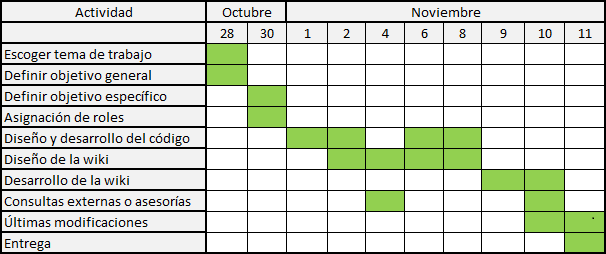
\includegraphics[width=0.75\textwidth]{imagenes/gantt_ejemplo}
        \caption{Diagrama de Gantt}
        \label{fig:diagrama-gantt}
    \end{figure}
\end{itemize}

\subsection{Diagrama de PERT}
\label{subsec:pert}

Proporciona una representación visual del cronograma de un proyecto y desglosa las tareas individuales.

\subsubsection{Conceptos fundamentales}

\begin{itemize}
    \item \textbf{Nodos:} Representan eventos (no actividades)
    \item \textbf{Flechas:} Actividades con duración
    \item \textbf{Camino crítico:} Ruta más larga (determina duración total)
\end{itemize}

\subsubsection{Elementos}

Este diagrama tiene los elementos de la \autoref{tab:tabladiapert}.

\begin{table}[htbp]
    \centering
    \begin{tabularx}{\textwidth}{|l|X|}
        \hline
        \textbf{Término}   & \textbf{Significado}                                                                          \\
        \hline
        D (Duración)       & Tiempo requerido para realizar la actividad                                                   \\
        \hline
        ES (Early Start)   & Primer momento posible de inicio                                                              \\
        \hline
        EF (Early Finish)  & Primer momento posible de fin                                                                 \\
        \hline
        LS (Late Start)    & Último momento posible de inicio                                                              \\
        \hline
        LF (Late Finish)   & Último momento posible de fin                                                                 \\
        \hline
        TF (Holgura Total) & Máximo retraso sin afectar proyecto                                                           \\
        \hline
        FF (Holgura Libre) & Máximo retraso sin afectar al \textquote{inicio temprano} de \textquote{sucesoras} inmediatas \\
        \hline
        Camino Crítico     & Secuencia de tareas más larga.
        Determinará la duración mínima del proyecto                    \\
        \hline
    \end{tabularx}
    \caption{Elementos del diagrama PERT}
    \label{tab:tabladiapert}
\end{table}

\subsubsection{Beneficios}

\begin{itemize}
    \item Identifica cuellos de botella
    \item Calcula probabilidades de cumplimiento
    \item Gestiona riesgos de tiempo
\end{itemize}


\section{Administración del Riesgo}
\label{sec:riesgos}
\begin{itemize}
    \item \textbf{RAE:} \textquote{Contingencia o proximidad de un daño}
    \item \textbf{Ingeniería del software:}
    \begin{itemize}
        \item Posibilidad de eventos imprevistos con impacto negativo en el proyecto
        \item Implica previsión del futuro, cambio y toma de decisiones
    \end{itemize}

    \item \textbf{Elementos clave:}
    \begin{itemize}
        \item \textbf{Fuente:} Origen del riesgo (ejemplo: nueva tecnología)
        \item \textbf{Evento:} Qué podría ocurrir (ejemplo: incompatibilidad)
        \item \textbf{Impacto:} Consecuencias (ejemplo: retraso 2 semanas)
    \end{itemize}
\end{itemize}

\subsection{Clasificación de Riesgos}
\label{subsec:clasificacion}

\begin{center}
    \begin{tabular}{p{3.5cm}p{9cm}}
        \toprule
        \textbf{Tipo de Riesgo} & \textbf{Descripción y Ejemplos} \\
        \midrule
        \textbf{Proyecto} &
        \begin{itemize}[leftmargin=*]
            \item Calendario o recursos insuficientes
            \item Ejemplo: Desarrollo por detrás de las metas acordadas con el cliente
        \end{itemize} \\
        \midrule
        \textbf{Técnico} &
        \begin{itemize}[leftmargin=*]
            \item Amenaza calidad o planificación
            \item ejemplo: Rendimiento inadecuado bajo carga máxima
        \end{itemize} \\
        \midrule
        \textbf{Producto} &
        \begin{itemize}[leftmargin=*]
            \item Incumplimiento expectativas usuario
            \item ejemplo: Interfaz poco intuitiva para usuarios finales
        \end{itemize} \\
        \midrule
        \textbf{Negocio} &
        \begin{itemize}[leftmargin=*]
            \item Problemas organizativos o de mercado
            \item ejemplo: Cambio en estrategia corporativa que reduce la prioridad del proyecto
        \end{itemize} \\
        \bottomrule
    \end{tabular}
\end{center}

\begin{center}
    \begin{tabular}{p{3.5cm}p{9cm}}
        \toprule
        \textbf{Tipo de Riesgo} & \textbf{Descripción y Ejemplos} \\
        \midrule
        \textbf{Tecnologías} &
        \begin{itemize}[leftmargin=*]
            \item Librerías obsoletas sin soporte
            \item Dependencias con licencias restrictivas
        \end{itemize} \\
        \midrule
        \textbf{Personal} &
        \begin{itemize}[leftmargin=*]
            \item Baja capacitación en tecnología clave
            \item Conflictos interpersonales en equipo
        \end{itemize} \\
        \midrule
        \textbf{Organizativos} &
        \begin{itemize}[leftmargin=*]
            \item Cambios frecuentes en liderazgo
            \item Presupuesto inestable
        \end{itemize} \\
        \midrule
        \textbf{Herramientas} &
        \begin{itemize}[leftmargin=*]
            \item Incompatibilidad entre entornos
            \item Bugs en software de testing
        \end{itemize} \\
        \midrule
        \textbf{Requisitos} &
        \begin{itemize}[leftmargin=*]
            \item Alcance no definido (scope creep)
            \item Requerimientos contradictorios
        \end{itemize} \\
        \midrule
        \textbf{Estimación} &
        \begin{itemize}[leftmargin=*]
            \item Subestimación de complejidad
            \item Falta de datos históricos
        \end{itemize} \\
        \bottomrule
    \end{tabular}
\end{center}

\subsection{Descripción de Riesgos}\label{subsec:descripcion-de-riesgos}

Para cada riesgo identificado, se recomienda recopilar la siguiente información:

\begin{itemize}
    \item \textbf{Descripción:} Cuál es el riesgo y cuál es su origen.

    \item \textbf{Prioridad (impacto):} \textit{alta} | \textit{media} | \textit{baja}

    \item \textbf{Probabilidad:} \textit{alta} | \textit{media} | \textit{baja}

    \item \textbf{Plan de acción:}
    \begin{itemize}
        \item Tipo: \textit{contingencia}, \textit{minimización} o \textit{prevención}
        \item Estrategia: \textit{soportar}, \textit{reducir el impacto}, \textit{evitar}
        \item Acciones planificadas: descripción específica de los pasos a seguir.
    \end{itemize}
    \item \textbf{Responsable:} Persona a cargo de la implementación del plan
    \item \textbf{Estado:} \textit{abierto} | \textit{cerrado}
\end{itemize}

\begin{exemplo}
    \textbf{Descripción:} Posible ausencia prolongada de una persona clave del equipo.

    \textbf{Impacto:} Alto

    \textbf{Probabilidad:} Promedio

    \textbf{Plan de contingencia:}
    \begin{itemize}
        \item Tipo: Contingencia
        \item Estrategia: Reducir el impacto
        \item Acciones: Documentar el trabajo clave y la capacitación cruzada dentro del equipo
    \end{itemize}

    \textbf{Responsable:} Coordinador del proyecto

    \textbf{Estado:} Abierto
\end{exemplo}

\subsection{Estrategias de Gestión de Riesgos}\label{subsec:estrategias-de-gestion-de-riesgos}

La gestión de riesgos puede adoptar diferentes enfoques según el momento oportuno para actuar sobre el riesgo:

\begin{itemize}
    \item \textbf{Estrategias reactivas:} Se actúa tras la materialización del riesgo, evaluando sus consecuencias y tomando medidas correctivas

    \item \textbf{Estrategias proactivas:} El riesgo se considera un posible evento futuro.
    Se establece un plan de contingencia para evitarlo o, en caso de ocurrir, minimizar su impacto
\end{itemize}

Un análisis temprano, sistemático y profundo de los riesgos favorece una estrategia proactiva global y reduce la ocurrencia de problemas imprevistos graves.

\medskip

\textbf{La gestión de riesgos} es el proceso continuo que permite:

\begin{itemize}
    \item Identificar riesgos potenciales
    \item Analizar su naturaleza e impacto
    \item Proponer soluciones antes de que se conviertan en problemas reales
\end{itemize}

Este proceso debe aplicarse continuamente durante todo el ciclo de vida del proyecto.

\begin{nota}
    La integración temprana de la gestión de riesgos en la planificación permite anticipar fallos, tomar decisiones más informadas y reducir costos inesperados.
\end{nota}

\subsection{Proceso de Gestión de Riesgos}
\label{subsec:proceso}
\deactivatequoting
\begin{center}
    \begin{tikzpicture}[node distance=1.5cm, auto]
        \tikzstyle{block} = [rectangle, draw, text width=6em, text centered, rounded corners, minimum height=4em]
        \tikzstyle{line} = [draw, -latex']

        \node [block] (identificar) {Identificación};
        \node [block, right of=identificar, node distance=4cm] (analizar) {Análisis};
        \node [block, right of=analizar, node distance=4cm] (planificar) {Planificación};
        \node [block, below of=analizar, node distance=3cm] (monitorear) {Seguimiento};

        \path [line] (identificar) -- (analizar);
        \path [line] (analizar) -- (planificar);
        \path [line] (planificar) |- (monitorear);
        \path [line] (monitorear) -| (identificar);
        \path [line] (monitorear) -- (analizar);
    \end{tikzpicture}
\end{center}
\activatequoting

\subsection{Actividades por fase}\label{subsec:actividades-por-fase}
\begin{itemize}
    \item \textbf{Identificación}: Listar riesgos potenciales
    \item \textbf{Análisis}: Calcular probabilidad/impacto, priorizar
    \item \textbf{Planificación}: Definir estrategias y planes de acción
    \item \textbf{Seguimiento}:
    \begin{itemize}
        \item Revisión mensual de riesgos activos
        \item Actualizar matriz de riesgos
        \item Activar planes de contingencia si es necesario
    \end{itemize}
\end{itemize}

\clearpage



    \chapter{Calidad}\label{ch:calidad}
    \minitoc
\begin{definicion}
    La calidad en software se define como un proceso eficaz que, al ser bien aplicado, crea un producto útil con valor mesurable tanto para los productores como para los usuarios.
\end{definicion}

La ingeniería de software tiene como objetivo garantizar esa calidad a lo largo de todo el ciclo de vida:

\begin{itemize}
    \item Planificación
    \item Diseño
    \item Desarrollo
    \item Pruebas
    \item Despliegue
    \item Mantenimiento
\end{itemize}


\section{Aseguramiento de la Calidad}\label{sec:aseguramiento-de-la-calidad}
\begin{definicion}
    Según la norma ISO/IEC 9126, la calidad de un producto software se puede evaluar mediante seis atributos principales:
\end{definicion}

\begin{enumerate}
    \item \textbf{Funcionalidad:} Grado en que el software cumple los requisitos funcionales esperados.
    \item \textbf{Confiabilidad:} Estabilidad del software ante fallos, por ejemplo, el tiempo medio de funcionamiento antes de un fallo.
    \item \textbf{Usabilidad:} Facilidad de uso para los usuarios.
    \item \textbf{Eficiencia:} Uso óptimo de los recursos disponibles (CPU, memoria, etc.).
    \item \textbf{Mantenibilidad:} Facilidad para modificar, corregir o mejorar el software.
    \item \textbf{Portabilidad:} Facilidad para trasladar el software entre diferentes entornos.
\end{enumerate}

\begin{nota}
    Existe un dilema clásico entre producir software rápido y barato o producir software de alta calidad, ya que la calidad requiere tiempo y recursos.
\end{nota}

\begin{nota}
    Los errores pequeños no detectados a tiempo pueden amplificarse y causar problemas mayores en fases posteriores, por lo que la detección temprana es fundamental.
\end{nota}

\subsection{Principios rectores de la calidad}\label{subsec:principios-rectores-de-la-calidad}
\begin{itemize}
    \item \textbf{Formulación.} La derivación de medidas y métricas de software apropiadas
    \item para la representación del software que se está construyendo.
    \item \textbf{Recolección. }Mecanismo que se usa para acumular datos requeridos para derivar las métricas formuladas.
    \item \textbf{Análisis.} El cálculo de métricas y la aplicación de herramientas
    \item matemáticas.
    \item \textbf{Interpretación.} Evaluación de las métricas resultantes para comprender la calidad de la representación.
    \item \textbf{Retroalimentación.} Recomendaciones derivadas de la interpretación de las métricas del producto, transmitidas al equipo de software.
\end{itemize}

\subsection{Atributos de las métricas}\label{subsec:atributos-de-las-metricas}
\begin{enumerate}
    \item \textbf{Medible. }Debe ser simple poder recolectar los datos que componen la métrica y realizar su cálculo.
    \item \textbf{Intuitiva.} Los usuarios de la métrica deben poder identificar su significado y su valor.
    \item \textbf{Objetiva.} Siempre debe producir resultados que no tengan ambigüedades.
    \item \textbf{Coherente.} El cálculo matemático de la métrica debe usar medidas que no conduzcan a combinaciones extrañas de unidades.
    \item \textbf{Tecnológicamente agnóstica.} Debe basarse en el modelo de requerimientos, el modelo de diseño o la estructura del programa en sí.
    \item \textbf{Accionable.} Debe proporcionar información que pueda conducir a un producto final de mayor calidad.
\end{enumerate}

\subsection{Control vs. Aseguramiento de la Calidad}\label{subsec:control-vs.-aseguramiento-de-la-calidad}

\begin{center}
    \begin{tabularx}{\textwidth}{|X|X|}
        \hline
        \textbf{Control de Calidad (QC)}                         & \textbf{Aseguramiento de Calidad (QA)}               \\
        \hline
        Reactivo                                                 & Proactivo                                            \\
        Detección y corrección de errores después de que ocurren & Prevención de errores mediante estándares y procesos \\
        Inspección de productos                                  & Mejora continua de procesos                          \\
        \hline
    \end{tabularx}
\end{center}

\subsection{Revisiones técnicas}\label{subsec:revisiones-tecnicas}

\begin{itemize}
    \item \textbf{Informales:} Conversaciones espontáneas, revisiones en escritorio; baja eficacia que mejora con listas de verificación.
    \item \textbf{Formales:} Reuniones estructuradas y preparadas; alta eficacia, más tiene un alto coste en tiempo y esfuerzo; se utiliza normalmente una muestra representativa.
\end{itemize}

\subsection{Revisiones durante el desarrollo}\label{subsec:revisiones-durante-el-desarrollo}

\begin{itemize}
    \item \textbf{Revisión de código:} Entre compañeros (pair review) para detectar errores y mejorar el aprendizaje del equipo.
    \item \textbf{Análisis estático de código:} Herramientas automáticas que detectan errores potenciales, complejidad y duplicaciones.
\end{itemize}

\subsection{Métricas de calidad (DORA Metrics)}\label{subsec:metricas-de-calidad-(dora-metrics)}

\begin{center}
    \begin{tabular}{|l|l|}
        \hline
        \textbf{Métrica}                  & \textbf{Significado}                                 \\
        \hline
        MTTR (Mean Time to Recover)       & Tiempo medio para recuperar un sistema tras un fallo \\
        MTBF (Mean Time Between Failures) & Tiempo medio entre fallos                            \\
        Disponibilidad                    & Proporción de tiempo que el sistema está disponible  \\
        \hline
    \end{tabular}
\end{center}

\begin{definicion}
    La disponibilidad se calcula con la fórmula:
    \[
        \text{Disponibilidad} = \frac{\text{MTBF}}{\text{MTBF} + \text{MTTR}} \cdot 100\%
    \]
\end{definicion}

\subsection{Buenas prácticas de desarrollo}\label{subsec:buenas-practicas-de-desarrollo}

\begin{itemize}
    \item \textbf{Clean Code} (Robert C. Martin - Uncle Bob):
    \begin{itemize}
        \item KISS: “Keep It Simple, Stupid”
        \item DRY: “Don’t Repeat Yourself”
        \item YAGNI: “You Aren’t Gonna Need It”
        \item SoC: “Separation of Concerns”
    \end{itemize}
    \item \textbf{Documentación:} Comentarios explicativos (no descriptivos), explicaciones en los commits y ejemplos de uso en tests.
    \item \textbf{Control de versiones:} Uso de herramientas como Git para seguir cambios y facilitar la colaboración.
\end{itemize}

\subsection{Métricas de desarrollo}\label{subsec:metricas-de-desarrollo}

\begin{center}
    \begin{tabular}{|l|l|}
        \hline
        \textbf{Métrica}                             & \textbf{Descripción}                       \\
        \hline
        Densidad de comentarios                      & \% de comentarios respecto al código total \\
        Duplicidad de código                         & Código repetido                            \\
        Cobertura de pruebas                         & \% de código ejecutado durante pruebas     \\
        Complejidad ciclomática                      & Mide rutas lógicas (condiciones y bucles)  \\
        IMS (Índice de Madurez del código(Software)) & Evalúa la estabilidad de una release       \\
        \hline
    \end{tabular}
\end{center}

\begin{definicion}
    La fórmula para calcular el IMS es:
    \[
        IMS = \frac{M_T - (F_a + F_c + F_d)}{M_T}
    \]
    Donde:
    \begin{itemize}
        \item $M_T$: Número total de pruebas planificadas.
        \item $F_a$: Fallos críticos encontrados.
        \item $F_c$: Fallos menores encontrados.
        \item $F_d$: Fallos detectados en desarrollo.
    \end{itemize}
\end{definicion}

\subsection{Deuda técnica}\label{subsec:deuda-tecnica}

\begin{definicion}
    Según Martin Fowler, la deuda técnica es una metáfora financiera: tomar atajos en el diseño genera un \textquote{interés} que se paga con mayor esfuerzo futuro.
    Se puede:
    \begin{itemize}
        \item Seguir pagando intereses (mantener mal diseño).
        \item Pagar el principal (refactorizar y mejorar).
    \end{itemize}
\end{definicion}

Se clasifica según dos ejes:

\begin{center}
    \begin{tabular}{|c|c|c|}
        \hline
        & \textbf{Temeraria}                              & \textbf{Prudente}                                    \\
        \hline
        \textbf{Deliberada}  & \textquote{No tenemos tiempo, entregamos ahora} & \textquote{Lo haremos rápido y mejoraremos después}  \\
        \hline
        \textbf{Inadvertida} & \textquote{¿Qué componentes tiene esto?}        & \textquote{Ahora sabemos cómo debería haberse hecho} \\
        \hline
    \end{tabular}
\end{center}


\section{Estrategias de Prueba}\label{sec:estrategias-de-prueba}

\subsection{Verificación vs. Validación}\label{subsec:verificacion-vs.-validacion}

\begin{center}
    %! suppress = LineBreak
    \begin{tabular}{|l|l|}
        \hline
        \textbf{Verificación}                     & \textbf{Validación}                         \\
        \hline
        ¿Construimos \textbf{bien} el producto?   & ¿Construimos el \textbf{producto correcto}? \\
        Garantía de implementación correcta       & Cumplimiento de requisitos del cliente      \\
        Incluye pruebas, revisiones, simulaciones & Incluye pruebas de aceptación y prototipos  \\
        \hline
    \end{tabular}
\end{center}

\subsection{Malas prácticas}\label{subsec:malas-practicas}

\begin{itemize}
    \item Suponer que hay partes que no se pueden probar.
    \item Que el desarrollador no haga pruebas.
    \item Aislar al equipo de pruebas.
    \item Involucrar a los testers solo al final.
\end{itemize}

\subsection{Estrategias de prueba (pirámide de pruebas)}\label{subsec:estrategias-de-prueba-(piramide-de-pruebas)}

Martin Fowler propone priorizar así:

\begin{enumerate}
    \item Pruebas unitarias (muchas, automáticas).
    \item Pruebas de integración.
    \item Pruebas de interfaz/aceptación (pocas, más caras de automatizar).
\end{enumerate}

\subsection{Dimensiones de la prueba}\label{subsec:dimensiones-de-la-prueba}

\begin{center}
    \begin{tabularx}{\textwidth}{|l|l|X|}
        \hline
        \textbf{Dimensión} & \textbf{Subdimensión}                   & \textbf{Descripción}                                    \\
        \hline
        Tipo               & Funcional / No funcional                & Comprobación de funciones / parámetros como rendimiento \\
        Granularidad       & Unitaria / Integración / Validación     & Nivel del sistema probado                               \\
        Alcance            & Progresión / Regresión / Smoke / Sanity & Cobertura funcional                                     \\
        Ejecución          & Manual / Asistida / Automática          & Nivel de automatización                                 \\
        Metodología        & Guiada / Exploratoria                   & Nivel de formalización                                  \\
        \hline
    \end{tabularx}
\end{center}

\subsection{Pruebas específicas}\label{subsec:pruebas-especificas}

\begin{itemize}
    \item \textbf{Unitarias:} \textbf{Caja blanca}.
    Son las pruebas más simples y frecuentes (sobre código individual).
    Uso de \emph{stubs} para módulos dependientes.
    Ejemplos: métodos, condiciones de frontera, errores.
    \item \textbf{Integración:} \textbf{Caja gris}.
    Pruebas de cómo interactúan los componentes.
    Importante la integración incremental (mayor control de errores).
    Puede ser ascendente o descendente.
    \item \textbf{Validación (aceptación):} \textbf{Caja negra}.
    Realistas y orientadas al usuario final.
    Difíciles de automatizar.
    Usadas en fases alfa y beta.
    \item \textbf{No funcionales:} Rendimiento, seguridad, recuperación, esfuerzo, despliegue, etc.
\end{itemize}


\section{Administración de la Configuración}\label{sec:administracion-de-la-configuracion}
\begin{definicion}
    Conjunto de actividades para gestionar los cambios durante el ciclo de vida del software, garantizando:
    \begin{itemize}
        \item Trazabilidad
        \item Control de versiones
        \item Información actualizada
    \end{itemize}

    Se diferencia del mantenimiento en que este aplica cambios, y la administración de configuración controla y registra dichos cambios.
\end{definicion}

\subsection*{Conceptos clave}
\begin{itemize}
    \item \textbf{Elemento de configuración (EC / ICS):} Unidad identificable que debe ser controlada (código, documentación, etc.).
    \item \textbf{Base de datos de configuración (BCD):} Lugar donde se almacenan los EC y sus versiones.
    \item \textbf{Línea base:} Versión estable y acordada de un conjunto de EC\@.
    \item \textbf{Cambio:} Modificación propuesta a un EC\@.
    \item \textbf{Control de cambios:} Proceso de evaluar y aprobar cambios.
\end{itemize}

\subsection{Ítems de Configuración (IC)}\label{subsec:items-de-configuracion-(ic)}
\begin{definicion}
    Cada uno de los elementos que comprenden toda la información
    producida como parte del proceso de software.
\end{definicion}
\begin{itemize}
    \item Programas de cómputo
    \item Productos de trabajo
    \item Contenido
\end{itemize}

\subsection{Sistema de Administración}\label{subsec:sistema-de-administracion}
\begin{itemize}
    \item \textbf{Elementos componentes:} Herramientas que permiten el acceso y gestión de cada ítem de configuración del software.
    \item \textbf{Elementos de proceso:} Acciones y tareas necesarias para realizar una gestión efectiva del cambio.
    \item \textbf{Elementos de construcción:} Herramientas que automatizan la compilación, empaquetado y generación de versiones correctas del software.
    \item \textbf{Elementos humanos:} Procesos y herramientas que utiliza el equipo para implementar de manera efectiva la administración de configuración.
\end{itemize}

\subsection{Repositorio ACS}\label{subsec:repositorio-acs}
\begin{definicion}
    Almacén centralizado o distribuido donde se gestionan los ítems de configuración.
\end{definicion}

\paragraph{Características clave:}
\begin{itemize}
    \item Control de versiones.
    \item Rastreo de dependencias entre componentes.
    \item Trazabilidad de requisitos y cambios.
    \item Apoyo a auditorías e inspecciones de calidad.
\end{itemize}

\subsection{Proceso de Administración de la Configuración}\label{subsec:proceso-de-administracion-de-la-configuracion}
\begin{enumerate}
    \item \textbf{Identificación:} Asignar nombres unívocos a los ítems de configuración.
    \item \textbf{Control de cambios:} Registrar, aprobar e implementar modificaciones.
    \item \textbf{Control de versiones:} Gestionar diferentes versiones de todos los objetos.
    \item \textbf{Auditoría:} Verificar que los cambios cumplen con los estándares establecidos.
    \item \textbf{Reporte de estado:} Informar del estado actual y del histórico de cambios.
\end{enumerate}

\subsection{Administración del contenido}\label{subsec:administracion-del-contenido}
\begin{itemize}
    \item \textbf{Subsistema de recopilación:} Permite almacenar y organizar el contenido asociado a cada Ítem de Configuración del Software (ICS).
    \item \textbf{Subsistema de administración:} Gestiona los cambios realizados sobre el contenido de cada ICS, manteniendo un histórico completo y trazable.
    \item \textbf{Subsistema de publicación:} Hace accesible el contenido relevante a los distintos interesados del proyecto, permitiendo su consulta o reutilización.
\end{itemize}

\subsection{Conflictos dominantes}\label{subsec:conflictos-dominantes}
\begin{itemize}
    \item \textbf{Contenido:} No está claro qué información debe formar parte del sistema de administración de configuración.
    \item \textbf{Personas:} El equipo desconoce las herramientas o procesos de ACS, o no sabe cuándo aplicarlos.
    \item \textbf{Escalabilidad:} A medida que crece el proyecto, se complica la gestión del gran volumen de cambios.
    \item \textbf{Políticas:} Faltan reglas claras sobre quién es responsable de llevar a cabo la administración de configuración y cómo aplicarla de manera coherente.
\end{itemize}




    \chapter{Mantenimiento}\label{ch:mantenimiento}
    \minitoc

    \section{Métricas de producto}\label{sec:tema-6.1---metricas-de-producto}
        \begin{definicion}
        \textbf{Métrica:} Medida cuantitativa del grado en que un sistema, componente o proceso posee un atributo determinado (IEEE Standard).
    \end{definicion}

    \subsection{Conceptos clave}\label{subsec:conceptos-clave}
    \begin{itemize}
        \item \textbf{Medida:} Un único dato.
        \item \textbf{Medición:} Recolección de varias medidas.
        \item \textbf{Indicador:} Combinación de métricas que proporciona comprensión sobre procesos, proyectos o productos.
    \end{itemize}

    \subsection{Principios de medición}\label{subsec:principios-de-medicion}
    \begin{enumerate}
        \item \textbf{Formulación:} Derivación de medidas apropiadas
        \item \textbf{Recolección:} Mecanismo para acumular datos
        \item \textbf{Análisis:} Cálculo de métricas con herramientas matemáticas
        \item \textbf{Interpretación:} Evaluación de resultados
        \item \textbf{Retroalimentación:} Recomendaciones al equipo
    \end{enumerate}

    \subsection{Atributos de métricas}\label{subsec:atributos-de-metricas}
    \begin{itemize}
        \item Medible
        \item Intuitiva
        \item Objetiva
        \item Coherente \item
        Tecnológicamente agnóstica
        \item Accionable
    \end{itemize}

    \subsection{Métricas específicas}\label{subsec:metricas-especificas}

    \begin{itemize}
        \item \textbf{Modelo de requisitos:}
        \[PF = conteo \cdot (0.65 + (0.01 \cdot \text{FAV}))\]
        \begin{itemize}
            \item Componentes:
            \begin{description}
                \item[Entradas externas (EE)]: Información que se origina de un usuario o se transmite desde otra aplicación.
                Se usan para actualizar archivos lógicos internos (ALI). Las entradas deben distinguirse de las consultas.
                \item[Salidas externas (SE)]: Datos derivados dentro de la aplicación que ofrecen información al usuario.
                \item [Consultas externas (CE)]: Entrada que da como resultado la generación de alguna respuesta (con frecuencia recuperada de un ALI).
                \item[Número de archivos lógicos internos (ALI)]:Agrupamiento lógico de datos que reside dentro de la frontera de la aplicación y se mantiene mediante entradas externas
                \item[Número de archivos de interfaz externos (AIE)]:
                Agrupamiento lógico de datos que reside fuera de la aplicación, pero que proporciona información que puede usar la aplicación.
                \item [Factor de ajuste de valor (FAV)]: Indica la complejidad del sistema en su conjunto en base a unas preguntas a las que se asigna un valor entre 0 (irrelevante) y 5 (esencial).
            \end{description}
        \end{itemize}

        \item \textbf{Diseño arquitectónico:}
        \begin{itemize}
            \item Complejidad de módulo: $S(i) = f^2_{out}(i)$, $D(i) = v(i) / (f_{out}(i) + 1)$
            \item Complejidad de sistema: $C(i) = S(i) + D(i)$
        \end{itemize}

        \item \textbf{Orientadas a clase (CK):}
        \begin{table}[!ht]
            \centering
            \caption{Métricas de la Suite CK}
            \label{tab:ck_metrics}
            \begin{tabularx}{\linewidth}{lX}
                \toprule
                \textbf{Acrónimo} & \textbf{Descripción}                                                                                                                                                          \\
                \midrule
                MPC               & Métodos Ponderados por Clase: Suma de las complejidades nominales de todos los métodos de una clase ($MPC = \sum c_i$), donde $c_i$ es la complejidad nominal de cada método. \\
                \addlinespace[0.3cm]
                PAH               & Profundidad del Árbol de Herencia: Longitud máxima desde el nodo de la clase actual hasta la raíz del árbol de herencia.                                                      \\
                \addlinespace[0.3cm]
                NDH               & Número de Hijos Directos: Cantidad de subclases que heredan directamente de la clase actual (subclases inmediatas).                                                           \\
                \addlinespace[0.3cm]
                FCOM              & Falta de Cohesión en Métodos: Número de pares de métodos que acceden a uno o más atributos de clase en común.                                                                 \\
                \bottomrule
            \end{tabularx}
        \end{table}

        \item \textbf{Código fuente:}
        \begin{itemize}
            \begin{table}[!ht]
                \centering
                \caption{Métricas de Halstead}
                \label{tab:halstead_metrics}
                \begin{tabular}{>{\bfseries}l l l}
                    \toprule
                    \multicolumn{1}{c}{\textbf{Símbolo}} &
                    \multicolumn{1}{c}{\textbf{Descripción}} &
                    \multicolumn{1}{c}{\textbf{Fórmula}} \\
                    \midrule
                    n1 & Número de operadores únicos    & Cantidad de tipos diferentes de operadores        \\
                    & en un programa                 &                                                   \\
                    \addlinespace

                    n2 & Número de operandos únicos     & Cantidad de tipos diferentes de operandos         \\
                    & en un programa                 &                                                   \\
                    \addlinespace

                    N1 & Frecuencia total de operadores & $N1 = \sum (\text{ocurrencias de cada operador})$ \\
                    &                                &                                                   \\
                    \addlinespace

                    N2 & Frecuencia total de operandos  & $N2 = \sum (\text{ocurrencias de cada operando})$ \\
                    &                                &                                                   \\
                    \bottomrule
                \end{tabular}
            \end{table}

            \item Longitud: $N = n_1 \log_2 n_1 + n_2 \log_2 n_2$
            \item Volumen: $V = N \log_2 (n_1 + n_2)$
        \end{itemize}

        \item \textbf{Pruebas:}
        \begin{itemize}
            \item Nivel de programa: $PL = 1 / ((n_1/2) \cdot (N_2/n_2))$
            \item Esfuerzo de prueba: $e = V / PL$
        \end{itemize}

        \item \textbf{Mantenimiento:}
        \begin{itemize}
            \item Índice de madurez: $IMS = (M_1 - (F_a + F_c + F_d)) / M_1$
        \end{itemize}

        \item \textbf{SLA/SLO/SLI:}
        \begin{itemize}
            \item SLA: Acuerdo con cliente (Ejemplo: disponibilidad >99.9\%)
            \item SLO: Objetivo específico dentro de SLA
            \item SLI: Medida real de cumplimiento
        \end{itemize}
    \end{itemize}

% todo: completar

    \section{Tipos de mantenimiento}\label{sec:tipos-de-mantenimiento}
    \subsection{Leyes de Lehman}\label{subsec:leyes-de-lehman}
\begin{itemize}
    \item \textbf{Ley del cambio continuo.} En un entorno real, un sistema debe necesariamente cambiar para mantener su utilidad.
    \item \textbf{Ley de complejidad creciente.} Cuando el sistema evoluciona se hace más complejo.
    Hay que tomar medidas para evitarlo.
    \item \textbf{Ley de evolución. }La evolución es un proceso autorregulado.
    El tamaño, tiempo entre versiones, errores detectados, etc., se mantienen en el tiempo.
    \item \textbf{Ley de estabilidad organizacional.} Durante el tiempo de vida del sistema su velocidad de desarrollo es constante e independiente de los recursos dedicados su desarrollo.
    \item \textbf{Ley de conservación de la familiaridad.} A medida que un sistema evoluciona todo lo que está asociado con ello debe mantener un conocimiento total de su contenido y su comportamiento.
    \item \textbf{Ley de crecimiento continuado. }La funcionalidad ofrecida por los sistemas tiene que crecer continuamente para
    mantener la satisfacción de los usuarios.
    \item \textbf{Ley de decremento de la calidad.} La calidad de los sistemas software comenzará a disminuir a menos que dichos
    sistemas se adapten a los cambios de su entorno de funcionamiento.
    \item \textbf{Ley de retroalimentación.} Los procesos de evolución incorporan sistemas de retroalimentación.
\end{itemize}

\subsection{Proceso de mantenimiento}\label{subsec:proceso-de-mantenimiento}
\begin{itemize}
    \item \textbf{Causas de modificación:}
    \begin{itemize}
        \item Nuevos requisitos/cambios solicitados
        \item Corrección de errores
    \end{itemize}

    \item \textbf{Incorporación al desarrollo:}
    \begin{itemize}
        \item Implementación formal u hotfixes
    \end{itemize}

    \item \textbf{Factores de esfuerzo:}
    \begin{itemize}
        \item Diseño del sistema
        \item  Mecanismos de prueba
        \item Documentación
        \item  Estabilidad del personal
    \end{itemize}
\end{itemize}

\subsection{Clasificación de mantenimiento}\label{subsec:clasificacion-de-mantenimiento}
\begin{tabular}{|l|l|l|p{6cm}|c|}
    \hline
    \textbf{Categoría} & \textbf{Tipo} & \textbf{Descripción}          & \textbf{Esfuerzo} \\
    \hline
    Evolutivo          & Perfectivo    & Añadir nuevas funcionalidades & 50\%              \\
    \hline
    & Adaptativo    & Adaptar a nuevos entornos     & 25\%              \\
    \hline
    & Preventivo    & Mejorar mantenibilidad futura & 5\%               \\
    \hline
    Tradicional        & Correctivo    & Corregir errores              & 20\%              \\
    \hline
\end{tabular}

\subsection{Release Notes}\label{subsec:release-notes}
\begin{itemize}
    \item \textbf{Contenido esencial:}
    \begin{itemize}
        \item Novedades
        \item Mejoras
        \item Correcciones de errores
    \end{itemize}
\end{itemize}

\subsection{Sistemas heredados}\label{subsec:sistemas-heredados}
\begin{itemize}
    \item \textbf{Problemas comunes:}
    \begin{itemize}
        \item Código espagueti
        \item  Falta de documentación
        \item Estructura deficiente
        \item Especificaciones ausentes
    \end{itemize}

    \item \textbf{Solución:} Ingeniería inversa
\end{itemize}

\subsection{Reingeniería de sistemas}\label{subsec:reingenieria-de-sistemas}
\begin{definicion}
    Reestructuración, reescritura o re-documentación sin cambiar funcionalidad.
\end{definicion}

\begin{itemize}
    \item \textbf{Ventajas:} Más económico que desarrollo nuevo • Reemplazo gradual
    \item \textbf{Factores coste:} Personal experto, herramientas disponibles
    \item \textbf{¿Por qué?:} Más barato que el desarrollo.
\end{itemize}

\subsection{Tipos de reingeniería}\label{subsec:tipos-de-reingenieria}
\begin{itemize}
    \item Traducción de código
    \item Ingeniería inversa
    \item Reestructuración
    \item Ingeniería hacia adelante
    \item Migración de datos
\end{itemize}

\subsection{Flujo de reingeniería}\label{subsec:flujo-de-reingenieria}
\begin{enumerate}
    \item Código fuente sucio $\rightarrow$ Reestructuración $\rightarrow$ Código limpio
    \item Extracción de abstracciones $\rightarrow$ Especificación inicial
    \item Refinamiento $\rightarrow$ Especificación final
\end{enumerate}



    \chapter*{Anexos}
    \addcontentsline{toc}{chapter}{Anexos}
    \phantomsection

    \clearpage


    \section*{Anexo 1: Explicación de la Administración de Configuración de Software (ACS)}
    \addcontentsline{toc}{section}{Anexo 1: Explicación de la Administración de Configuración de Software (ACS)}
    \phantomsection

    \begin{multicols}{2}

        \begin{cajaazul}[¿Qué es ACS?]
            La Administración de Configuración de Software (ACS) es un conjunto de \textbf{procesos y herramientas} para gestionar los \textbf{cambios} en productos software durante todo su ciclo de vida.

            Va más allá de controlar solo versiones, integrando \textbf{documentación, dependencias, auditorías y trazabilidad}.
        \end{cajaazul}

        \vspace{0.5em}

        \begin{cajaverde}[Componentes principales]
            \begin{itemize}[leftmargin=*]
                \item \textbf{Control de versiones}: Histórico y gestión de versiones.
                \item \textbf{Gestión de dependencias}: Control de relaciones entre componentes.
                \item \textbf{Gestión de cambios}: Registro, planificación y aprobación.
                \item \textbf{Auditoría y trazabilidad}: Seguimiento detallado de cambios.
            \end{itemize}
        \end{cajaverde}

        \vspace{0.5em}
        \deactivatequoting
        \begin{cajanaranja}[Diferencias con Git]
            \begin{itemize}[leftmargin=*]
                \item \textbf{Alcance mayor}: Incluye código, documentación, requisitos, configuraciones\ldots
                \item \textbf{Procesos integrados}: Control de flujos y aprobaciones.
                \item \textbf{Trazabilidad}: Desde requisitos hasta entregables.
            \end{itemize}
        \end{cajanaranja}
        \activatequoting
        \vspace{0.5em}

        \begin{cajarosa}[Beneficios]
            \begin{itemize}[leftmargin=*]
                \item Mejora la calidad y estabilidad.
                \item Facilita el trabajo en equipos grandes.
                \item Reduce errores por cambios no controlados.
                \item Permite auditorías y cumplimiento.
            \end{itemize}
        \end{cajarosa}

        \vspace{0.5em}

        \begin{cajaroja}[¿Por dónde empezar?]
            \begin{itemize}[leftmargin=*]
                \item Usa un sistema de control de versiones (ej.\ Git).
                \item Documenta los elementos de configuración.
                \item Define políticas y procesos claros.
                \item Usa herramientas de seguimiento (p.ej.\ Jira).
                \item Forma al equipo en buenas prácticas.
            \end{itemize}
        \end{cajaroja}

    \end{multicols}

    \vspace{1em}
    \begin{center}
        \small\textit{Este anexo es una introducción visual y resumida para entender la Administración de Configuración de Software.}
    \end{center}


\end{document}
